\documentclass[compress, smaller, serif, 9pt]{beamer}

%TODO: change the notation of the dimension d->p to be consistent with the other lectures !!
%TODO: change the polynomial regression examples plot with those generated for the ML1A course <- done



\mode<presentation>
{
  \usetheme{Montpellier}
  %\setbeamercovered{transparent}
  % or whatever (possibly just delete it)
}
% or whatever
%\setbeamertemplate{footline}[frame number]
\beamertemplatenavigationsymbolsempty
\beamertemplatetransparentcovereddynamic

\usepackage[english,frenchb]{babel}
\usepackage[utf8]{inputenc}
% or whatever
%\setbeamertemplate{footline}[frame number]
\beamertemplatenavigationsymbolsempty
\beamertemplatetransparentcovereddynamic
\usefoottemplate{%
       \tinycolouredline{blue!03}%
       {
           \hspace{11.5cm}{\color{black!50} {\insertframenumber $/$ \inserttotalframenumber} \hfill}
       }%
}


% Definitions
%\input{def}
% Raccourcis
%\input{raccourci}

% Beamer settings
%\setbeamercolor{structure}{fg=myem!120}
%\setbeamercolor{example}{bg=LightYell,fg=StroYell}

% \setbeamercolor{alerted text}{fg=lightred}
% \setbeamertemplate{blocks}[rounded][shadow=true]
% \newcommand{\exampletext}[1]{{\usebeamercolor[fg]{example text} #1}}
% \newcommand{\structuretext}[1]{{\usebeamercolor[fg]{structure} #1}}
% \usefonttheme[onlymath]{serif}
% \renewcommand{\thefootnote}{\fnsymbol{footnote}}

%\setbeamerfont{sidebar}{5pt}

\usepackage{amssymb}
%\usepackage[T1]{fontenc}
\usepackage{amsmath,amsthm,bm}
\usepackage{pgf}


\graphicspath{{./Figs/S01/}}

\usepackage[normal]{subfigure}
\newcommand{\goodgap}{%
    \hspace{\subfigtopskip}%
    \hspace{\subfigbottomskip}}

% les macros
\newcommand{\exampletext}[1]{{\usebeamercolor[fg]{example text} #1}}
\newcommand{\structuretext}[1]{{\usebeamercolor[fg]{structure} #1}}

\newcommand{\bydef}{\stackrel{{def}}{=}}
\newcommand{\ici}{\tcb{$\blacktriangleright \;$}}
\newcommand{\icir}{\alert{$\blacktriangleright \;$}}
\newcommand{\iciex}{\exampletext{$\blacktriangleright \;$}}
\usepackage{pifont}
\newcommand{\doigt}{\structuretext{\noindent \Pisymbol{pzd}{43}}}
\newcommand{\doigtr}{\alert{\noindent \Pisymbol{pzd}{43}}}
\newcommand{\doigtex}{{\exampletext{\noindent \Pisymbol{pzd}{43}}}}


\setbeamerfont{block title}{size={\normalsize}}


\title[Statistical Learning]{Machine/Statistical Learning}

\subtitle{Lecture 1: Introduction}


\author[Florent Chatelain]{Florent Chatelain}
\institute{Filière SICOM, 3A}
%\logo{\includegraphics[width=.2\textwidth]{logoE3}}
\date{2016-17}


%

\begin{document}

\maketitle


\section{Organization}

\begin{frame}
  \frametitle{Organization}

\begin{block}{Volume}
\begin{itemize}
 \item 6 $\times$ 2h lecture sessions
 \item 2 $\times$ 4h Lab sessions
 \item Evaluation: exam (2h)
\end{itemize}
\end{block}

\begin{block}{Objectives}
\begin{itemize}
 \item model/algorithm analysis for supervised/unsupervised learning
 \item application of these algorithms on different datasets (artificial intelligence, bioinformatics, vision, etc ...)
\end{itemize}
\end{block}

\end{frame}

\begin{frame}
  \frametitle{Organization}
\begin{block}{Lectures}
\begin{itemize}
 \item[S01] Introduction
 \item[S02] Supervised linear methods 
 \item[S03] Logistic regression
 \item[S04] Support Vector Machine
 \item[S05] Unsupervised classification: clustering
 \item[S06] Dictionary Learning
\end{itemize}
\end{block}

\begin{block}{Labs}
\begin{itemize}
 \item[L01] Supervised methods, model selection and validation
 \item[L02] Unsupervised classification (clustering)
\end{itemize}
\end{block}


\end{frame}


\section{Références}

\begin{frame}
\begin{block}{Reference books}
\begin{thebibliography}{9}
\setbeamertemplate{bibliography item}[book]
\bibitem{A} Trevor Hastie, Robert Tibshirani et Jerome Friedman (2009)\\
\normalcolor{The Elements of Statistical Learning (2nd Edition)}\\
\color{gray}{\it Springer Series in Statistics}
\bibitem{B} Christopher M. Bishop (2007) \\
\normalcolor{Pattern Recognition and Machine Learning}\\
\color{gray}{\it Springer}
\bibitem{C}
Richard O. Duda, Peter E. Hart et David G. Stork (2001)\\
\normalcolor{Pattern classification (2nd edition)}\\
\color{gray}{\it Wiley}
\end{thebibliography}
\end{block}

\begin{block}{\normalcolor{Supplementary materials, datasets, online courses, ...}}
\begin{thebibliography}{9}
\setbeamertemplate{bibliography item}[online]
\bibitem{A} \url{http://www-stat.stanford.edu/~tibs/ElemStatLearn/}
\bibitem{B} {\small \url{http://research.microsoft.com/en-us/um/people/cmbishop/prml/} }
%\bibitem{C} \url{http://www.math.u-bordeaux.fr/~fcaron/}
\bibitem{D} \url{https://www.coursera.org/course/ml} \color{gray}{\scriptsize \it very popular MOOC (Andrew Ng)}
\bibitem{E} \url{https://work.caltech.edu/telecourse.html} \color{gray}{\scriptsize \it more involved MOOC (Y. Abu-Mostafa)}
\end{thebibliography}
\end{block}

\end{frame}

\section{Examples}
\begin{frame}
  \frametitle{Examples}
\begin{block}{Recognition of handwritten digits (US postal envelopes)}
\begin{center}
  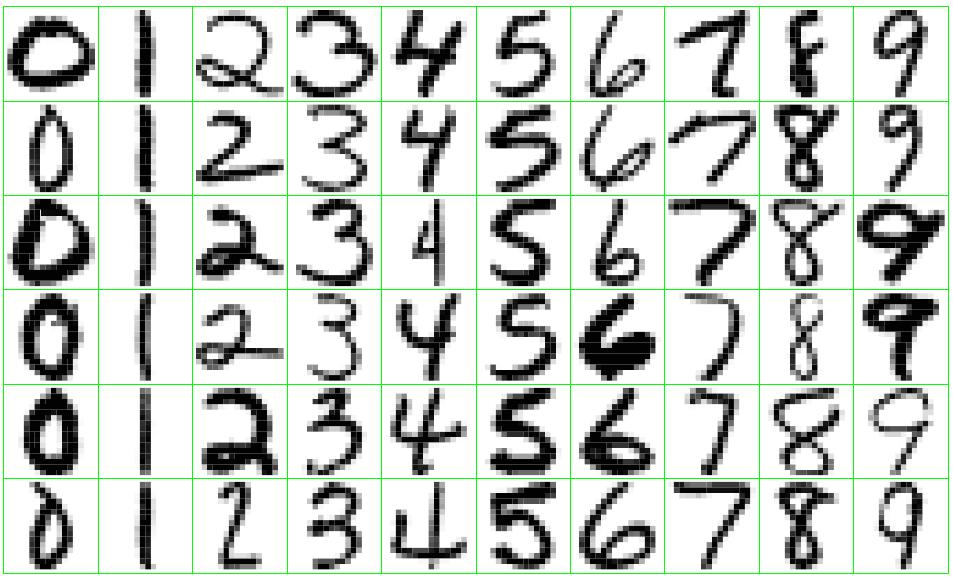
\includegraphics[width=.5\textwidth]{ex_handwriten.jpg}
\end{center}
\begin{itemize}
\item[\doigt] Predict the class (0,...,9) of each sample from an image of 
$16\times 16$ pixels, with a pixel intensity coded from $0$ to $255$
\item Low error rate to avoid wrong allocations of mails!
\end{itemize}
\end{block}
\begin{center}
 \alert{Supervised classification }
\end{center}
\end{frame}

\begin{frame}
  \frametitle{Examples}
\begin{block}{Spams Recognition}
\begin{center}
  
\includegraphics[width=.8\textwidth]{ex_spams.jpg}
\end{center}
\begin{itemize}
\item[\doigt] 
Define a model to predict whether an email is spam or not
\item Low error rate to avoid deleting useful messages, or filling the mailbox with useless emails
\end{itemize}
\end{block}
\begin{center}
 \alert{supervised classification}
\end{center}

\end{frame}

\begin{frame}
  \frametitle{Examples}
\begin{block}{Disaggregation/Prediction of appliance's, or industrial, load}
\begin{center}
  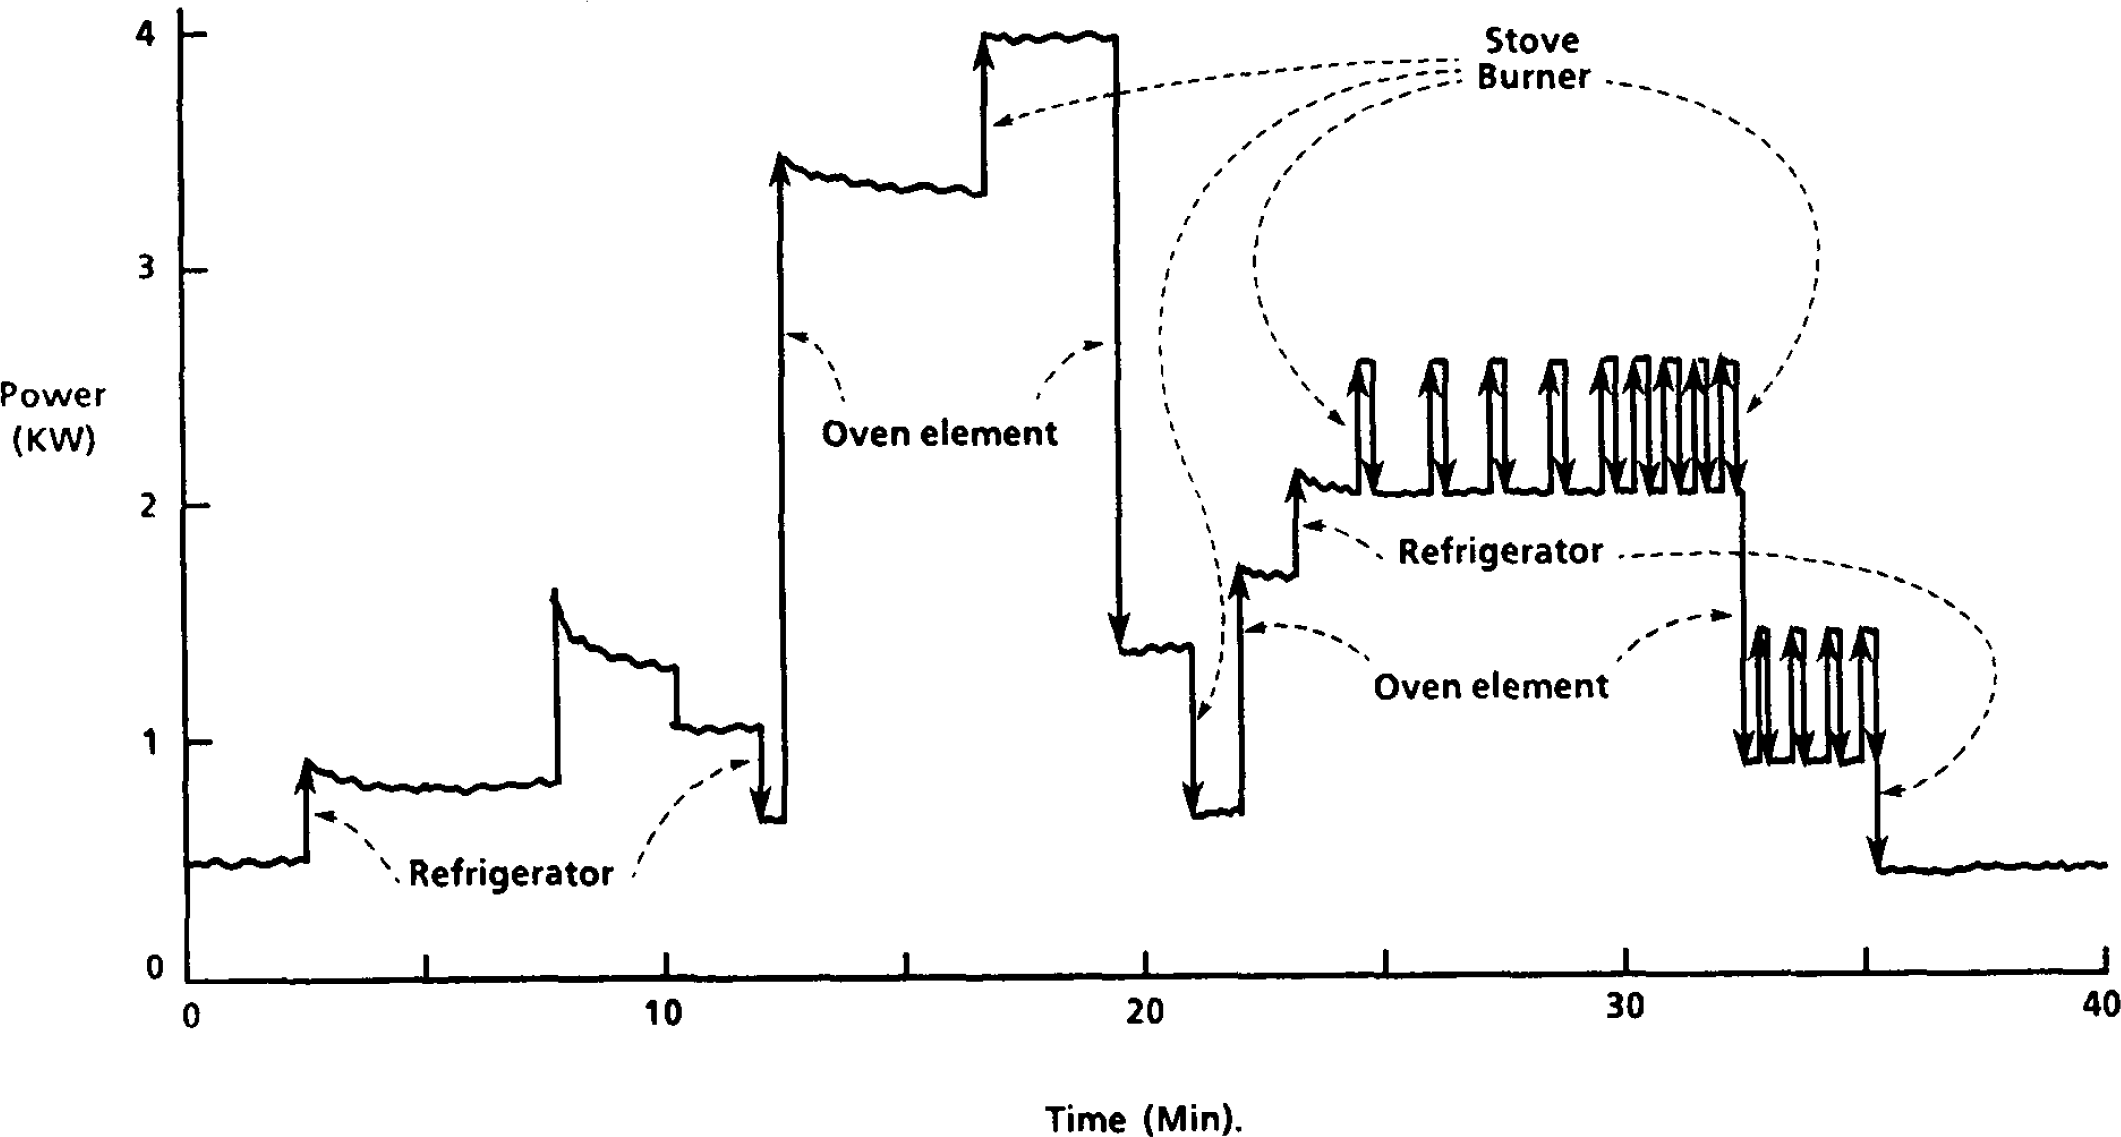
\includegraphics[width=.7\textwidth]{ex_CDC.png}
\end{center}
\begin{itemize}
\vspace{-5mm}
\item[\doigt] Individual appliance recognition from load curves
\item[\doigt] Predict the energy consumption
%à partir de courbes de charges apprise et de données sur l'habitation
%\item Taux d'erreur faible afin d'éviter de détecter des usages inexistants, ou
%de ne pas sur/sous dimensionner le réseau
\end{itemize}
\end{block}
\begin{center}
 \alert{supervised or unsupervised classification}
\end{center}

\end{frame}



\begin{frame}
  \frametitle{Examples}
\begin{block}{DNA-microarrays}
\begin{center}
  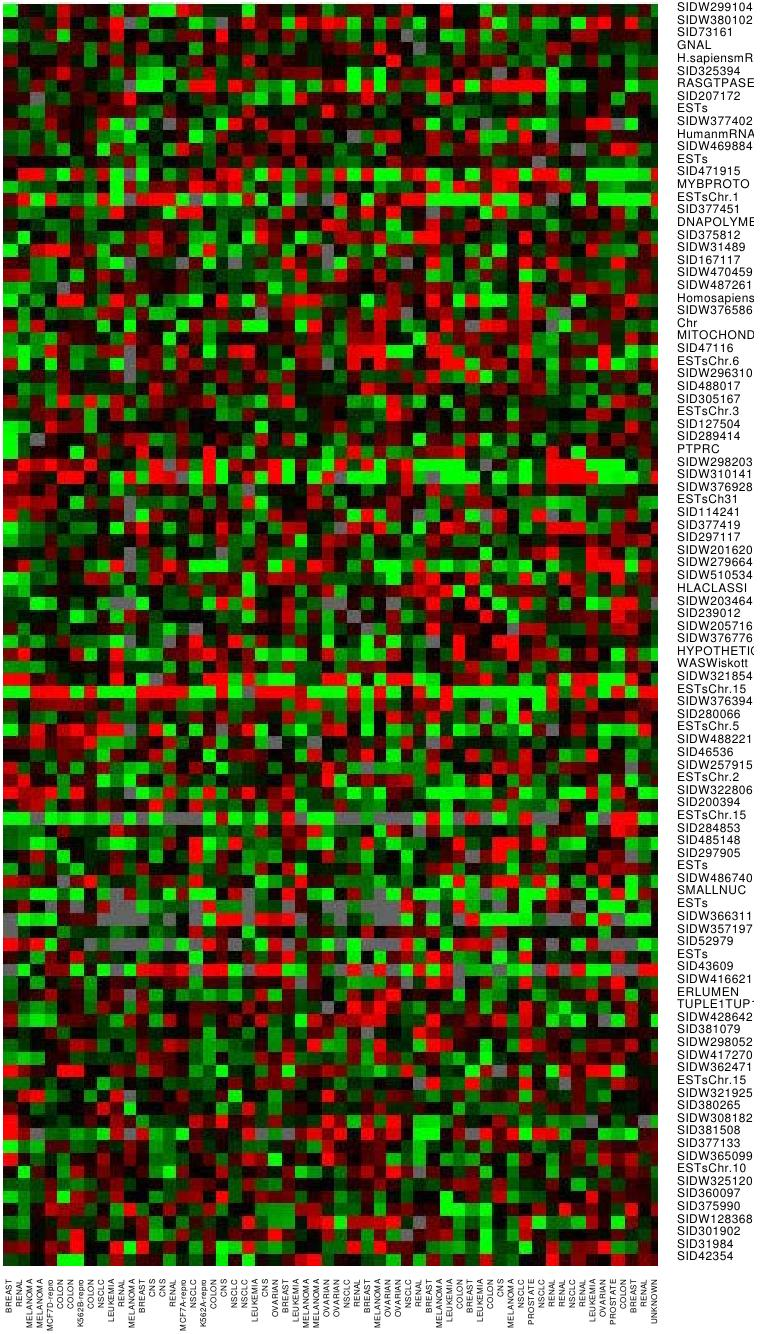
\includegraphics[angle=90, origin=c, width=.6\textwidth]{ex_biopuce.jpg}
\end{center}
\vspace{-20mm}
\begin{itemize}
\item Genes expression dataset fore several thousand individual genes (columns) and tens of samples  (rows)
\item[\doigt] Classification of genes (resp. samples)  with similar expression profiles across samples (resp. genes)
\end{itemize}
\end{block}
\begin{center}
 \alert{unsupervised classification}
\end{center}
\end{frame}

\section{Definitions}

\begin{frame}
  \frametitle{Definitions}
\begin{block}{Variable terminology}
\begin{itemize}
 \item observed data referred to as {\em input} variables, {\em predictors} or {\em features} $\leftarrow$ usually denoted as $X$
 \item data to predict referred to as {\em output} variables, or {\em responses}  $\leftarrow$ usually denoted as $Y$
\end{itemize}
\end{block}

\begin{block}{Type of prediction problem: regression vs classification}
Depending on the type of the {\em output} variables
\begin{itemize}
 \item when $Y$ are \structuretext{quantitative} data (continuous variables, e.g. electrical load curve values) $\leftarrow$ \structuretext{regression}
 \item when $Y$ are \structuretext{categorical} data (discrete qualitative variables, e.g. handwritten digits $Y\in \{0,\ldots,9\}$) $\leftarrow$ \structuretext{classification}
\end{itemize}\medskip

Two very close problems. In this course, mainly classification tasks
\end{block}
\end{frame}




\begin{frame}
  \frametitle{Prediction problem}
\begin{block}{Assumptions}
\begin{itemize}
 \item couples of input and output variables $(X_i,Y_i)$ are i.i.d.
 \item input variables $X_i$ are vectors in $\mathbb{R}^p$:
 \begin{align*}
  X_i= \left(X_{i,1}, \ldots, X_{i,p} \right)^T \in \mathcal{X} \subset \mathbb{R}^p
 \end{align*}
 \item output variables $Y_i$ take values:
 \begin{itemize}
  \item in $\mathcal{Y \subset \mathbb{R}}$ (regression)
  \item in a finite set $\mathcal{Y}$ (classification)
\end{itemize}
\end{itemize}
\end{block}
\begin{block}{Prediction rule}
 function of prediction / rule of classification $\equiv$ function $f: \  \mathcal{X} \rightarrow \mathcal{Y}$   
\end{block}
\end{frame}

\begin{frame}
  \frametitle{Supervised or unsupervised learning}
  
\begin{block}{}
\structuretext{Training set} $\equiv$ available sample  $\mathcal{T}$ to learn the prediction rule $f$ \medskip 

For a sized $n$ training set, different cases:
\begin{itemize}
 \item \structuretext{Supervised learning}:  $ \mathcal{T} \equiv \left( (X_1,Y_1), \ldots, (X_n,Y_n) \right)$ input/output couples are available to learn 
 the prediction rule $f$
 \item \structuretext{Unsupervised learning}: $ \mathcal{T} \equiv \left( X_1, \ldots, X_n \right)$ only the inputs  are available 
 \item \structuretext{Semi-supervised}: mixed scenario (often encountered in practice, but less information than in the supervised case)
\end{itemize}
\end{block}

During this course:
\begin{itemize}
 \item S02 $\rightarrow$ S04 and Lab1 devoted to supervised learning (more interpretable results, abundant literature)
 \item S05 $\rightarrow$ S06 and Lab2 devoted to unsupervised learning
\end{itemize}

\end{frame}



\section{Statistical Decision Theory}

\subsection{Prediction function / Loss function}

\begin{frame}
  \frametitle{Prediction problem}
  We seek a regression function / classification rule for  \alert{accurate} predictions $f(X)$ 
  of new elements $Y$ given $X$.
  \begin{description}
   \item[Problem:] \alert{accurate ??}
   \item[Solution:] Introduction of a loss function:
   \begin{align*}
    L: \quad & \mathcal{Y} \times \mathcal{Y} \rightarrow \mathbb{R}^+,
   \end{align*}
   in order to penalize the prediction errors:
\begin{align*}
    L (Y, f(X) ) &
    \begin{cases}= 0 \textrm{ if } f(X)=Y,\\
     \ge 0 \textrm{ otherwise},
     \end{cases}
   \end{align*}
  \end{description}


  \begin{block}{Two useful loss functions}
  \begin{enumerate}
   \item Quadratic cost: $ L (Y, f(X) ) = \left( Y - f(X) \right)^2$,\\
   \item $0-1$ cost~: \vspace{-3mm} $$
 L (Y, f(X) ) = \begin{cases}
                                         0 \textrm{ if } | Y - f(X) | < \epsilon \quad ( \epsilon>0 \textrm{ arbitrarily small}),\\
                                         1 \textrm{ otherwise}
                                        \end{cases}$$
   Rk: for a classification pb,  $ L (Y, f(X) ) = 0$ if $Y = f(X)$, $1$ otherwise
  \end{enumerate}
\end{block}
\end{frame}

\subsection{Error rate}

\begin{frame}
  \frametitle{Error rate}
  \begin{block}{True error}
   The {\it true error rate} w.r.t. a prediction function $f$
   and a loss function $L$ is defined as
   \begin{align*}
    \mathcal{E}[f]&= E_{X,Y} \left[ L\left(Y,f(X) \right) \right],\\
    &= \int  L\left(y,f(x) \right) dP(x,y),
   \end{align*}
  where $P(x,y)$ is the joint probability measure of $(X,Y)$.
  \end{block}
  \begin{block}{Training error}
   The {\it training error rate} w.r.t. a prediction function $f$, 
   a loss function $L$, and a training dataset  $(X_1,Y_1), \ldots,(X_N,Y_N)$
   is defined as the empirical mean
   \begin{align*}
    \hat{\mathcal{E}}_N[f]&= \frac{1}{N} \sum_{i=1}^N  L\left(Y_i,f(X_i) \right)
   \end{align*}
  \end{block}
\end{frame}

\begin{frame}
  \frametitle{Error rates for usual loss functions}
  \begin{block}{Quadratic cost (rather for regression)}
   \begin{itemize}
   \item True error rate  $\rightarrow${\it Mean Squared Error} (MSE)
   \begin{align*}
    \mathcal{E}[f]&= E_{X,Y} \left[ \left(Y-f(X) \right)^2 \right]
    = \int  \left(y-f(x) \right)^2 dP(x,y),
   \end{align*}
   \item Training error rate  $\rightarrow$ {\it Residual Sum of Squares} (RSS)
   \begin{align*}
    \hat{\mathcal{E}}_N[f]&= \frac{1}{N} \sum_{i=1}^N \left(Y_i -f(X_i)\right)^2
   \end{align*}
   \end{itemize}
  \end{block}
  \begin{block}{$0-1$ cost (rather for classification)}
   \begin{itemize}
   \item  True error rate:
   \vspace{-6mm}
   \begin{align*}
                  \qquad  \qquad          \qquad    \mathcal{E}[f]& = \Pr\left( \left| Y-f(X) \right|> \epsilon  \right),\\
                              &=  \Pr\left(Y \ne f(X)\right) \leftarrow  \textrm{ classification}
                             \end{align*}
   \item Training error rate:
   \vspace{-9mm}
   \begin{align*} \qquad     
    \hat{\mathcal{E}}_N[f]&  = \frac{1}{N} \sum_{i=1}^N 1_{|Y_i -f(X_i)| > \epsilon}
    %=  \frac{1}{N} \sum_{i=1}^N&  1_{Y_i \ne f(X_i)}\leftarrow  \textrm{ classification}
    \end{align*}
   \end{itemize}
  \end{block}
\end{frame}

\begin{frame}
  \frametitle{Example of true error rate}
  \begin{center}
    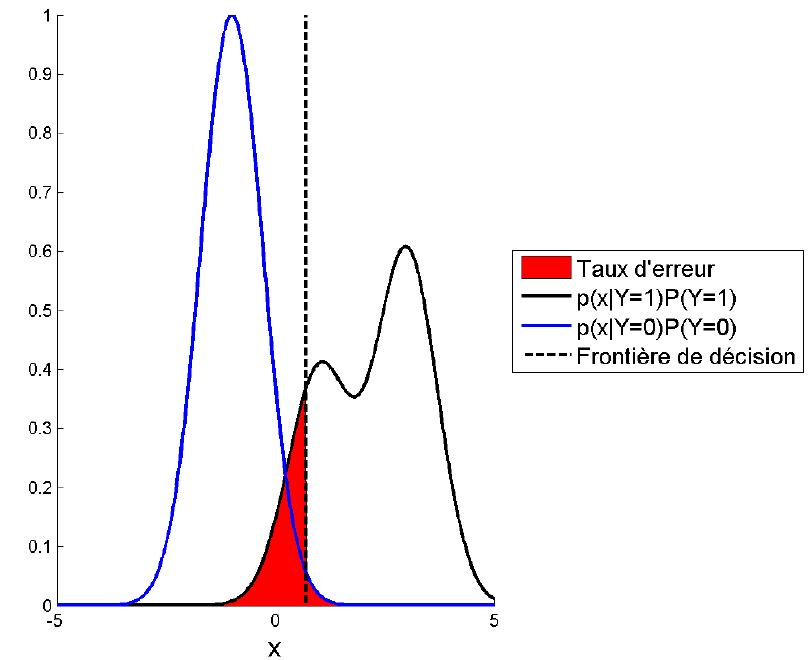
\includegraphics[width=.8\textwidth]{ex_taux_erreur.jpg}
  \end{center}
\end{frame}

\subsection{Regression}

\begin{frame}
  \frametitle{Optimal prediction for the regression problem}
  \begin{itemize}
   \item $Y \in \mathcal{Y} \subset \mathbb{R} \quad \leftarrow$ continuous domain
  \end{itemize}

  \begin{block}{Definition}
  The conditional expectation of $Y$ given $X=x$ is defined as:
   \begin{align*}
    E[Y | X=x]&= \int_{\mathcal{Y}} y \,dP( Y | X = x) = \int_{\mathcal{Y}} y\, p( y | X = x) dy,
   \end{align*}
   and we denote as $E[Y | X]$ the associated random variable.
  \end{block}
 \begin{block}{Theorem}
  The regression function defined as the conditional expectation
   $f_{\textrm{MMSE}}(x) = E[Y | X=x]$
  is optimal in the quadratic loss sense:
   for any rule $f$, $\mathcal{E}[f] \ge \mathcal{E}[f_{\textrm{MMSE}}]$.
 \end{block}
 {\scriptsize
  \begin{block}{Remarks}
   \begin{itemize}
    \item $f_{\textrm{MMSE}}(X) \equiv$ {\it Minimum Mean Squared Errors} (MMSE) estimator
    \item In real-word applications,  the distribution of $(X,Y)$ is unknown $\Rightarrow$ no analytical expression  of $f_{\textrm{MMSE}}(X)$. 
    But useful reference on academic examples.
   \end{itemize}
 \end{block}
 }
\end{frame}

\begin{frame}
  \frametitle{Optimality of the Conditional Expectation}
 \vspace*{-5mm}
  \begin{block}{\small Proof}
\vspace*{-5mm}{\scriptsize
 \begin{align*}
  \mathcal{E}[f]&= E_{X,Y}\left[ ( Y - f(X) )^2 \right] =
  \int_{\mathcal{X} \times \mathcal{Y}} ( y - f(x) )^2 p(x ,y )  dx dy,\\
  &= \int_{\mathcal{X}} \underbrace{\int_{\mathcal{Y}}  ( y - f(x) )^2 p( y | x )   dy}_{A_x}  \, p(x) dx. \vspace*{-5mm}
 \end{align*}

 To minimize $\mathcal{E}[f]$, it is sufficient to get a pointwise minization of  $A_x$  $\forall \ x \in \mathcal{X}$~:
  \begin{align*}
  A_x &= E_{Y|X=x} \left[ ( Y - f(x) )^2 |X=x \right]
  = E_{Y|X=x} \left[ \left( Y - E[Y|X=x] + E[Y|X=x] - f(x) \right)^2 |X=x \right],\\
  &= E_{Y|X=x} \left[ ( Y - E[Y|X=x])^2 \right] +  E_{Y|X=x} \left[ ( E[Y|X=x] - f(x) )^2 \right] \\
  &\quad +
  2 \underbrace{E_{Y|X=x} \left[  ( Y - E[Y|X=x]) ( E[Y|X=x] - f(x) )  \right]}_{B_x}.\vspace*{-15mm}
  \end{align*}\vspace*{-6mm}
  But
   \begin{align*}
  B_x&= E_{Y|X=x} \left[  ( Y - E[Y|X=x]) \right] ( E[Y|X=x] - f(x) ),\\
  &= ( E[Y|X=x] - E[Y|X=x]) ( E[Y|X=x] - f(x) ) = 0,
  \end{align*}
  thus
  $A_x= E_{Y|X=x} \left[ ( Y -f_{\textrm{MMSE}}(x) )^2 \right] + ( f_{\textrm{MMSE}}(x)  - f(x) )^2  \ge E_{Y|X=x} \left[ ( Y -f_{\textrm{MMSE}}(x) )^2 \right]$
.\\ Finally $\mathcal{E}[f]= E_X[A_X] \ge E_X\left[ E_{Y|X} \left[ ( Y -f_{\textrm{MMSE}}(X) )^2 \right] \right] = \mathcal{E}[f_{\textrm{MMSE}} ]$
 \qed}
 \end{block}

\end{frame}


\subsection{Classification}
\begin{frame}
  \frametitle{Bayes classifier}
  \begin{itemize}
   \item $Y \in \mathcal{Y} \quad \leftarrow$ discrete domain
  \end{itemize}

  \begin{block}{Definition}
  The Bayes classification rule $f^{\ast}$ is defined as
   \begin{align*}
    f^{\ast}(x)= \arg \max_{k \in\mathcal{Y}  } \Pr( Y= k | X=x).
   \end{align*}
   The associated error rate  $\mathcal{E}[f^{\ast}]$ is refered to as the \color{blue}{Bayesian error rate}
  \end{block}
 \begin{block}{Theorem}
 The Bayes classification rule $f^{\ast}$ is optimal in the $0-1$ loss sense: 
   for any rule $f$, $\mathcal{E}[f] \ge \mathcal{E}[f^{\ast}]$.
 \end{block}
  \begin{block}{Remarks}
   \begin{itemize}
    \item $f^{\ast}(X) \equiv$  {\it maximum a posteriori} (MAP) estimate
    \item In real-word applications,  the distribution of $(X,Y)$ is unknown $\Rightarrow$ no analytical expression  of $f^{\ast}(X)$. 
    But useful reference on academic examples.
   \end{itemize}

 \end{block}
\end{frame}

\begin{frame}
  \frametitle{Optimality of the Bayes classifier}
\begin{block}{Proof}
 \begin{align*}
  \mathcal{E}[f]= \Pr( Y \ne f(X) ) = \int_\mathcal{X} \underbrace{\Pr( Y \ne f(X) |X=x )}_{A_x} p(x) dx,
 \end{align*}
 where
  \begin{align*}
  A_x &= \Pr( Y \ne f(x) |X=x ),\\
  &= 1 - \Pr( Y = f(x) |X=x ).
 \end{align*}
 To minimize $\mathcal{E}[f]$, it is sufficient to get  a pointwise minization of $A_x$ for $x \in \mathcal{X}  $
 $\Leftrightarrow$
 equivalent to maximize $\Pr( Y = f(x) |X=x )$ \qed
 \end{block}
\end{frame}

\begin{frame}
  \frametitle{Exercise}
\begin{block}{Statement}
We consider the following binary classification problem:
\begin{itemize}
 \item $Y \in \{0,1\}$, $X \in [0,5]$, $\Pr(Y=0)=\Pr(Y=1)=\frac{1}{2}$, and
 \begin{align*}
  X|Y=0 &\sim \mathcal{U}\left([0,2]\right),\\
  X|Y=1 &\sim \mathcal{U}\left([1,5]\right)
 \end{align*}
\end{itemize}
\begin{enumerate}
 \item Compute the true error rates for the following classifiers:
 \begin{itemize}
 \item $f_1(X) = 0$ if $X \le 0$, $1$ otherwise
 \item $f_2(X) = 0$ if $X \le 2$, $1$ otherwise
 \item $f_3(X) = 0$ if $X \le 4$, $1$ otherwise
\end{itemize}
\item Find the Bayes classifier expression and its error rate. 
\end{enumerate}
 \end{block}
\end{frame}

\begin{frame}
  \frametitle{Exercise}
\begin{block}{Sketch of correction}
\begin{enumerate}
 \item Applying, the law of total probability, it comes that 
 \begin{itemize}
 \item $\Pr( Y \ne f_1(X) ) = \frac{1}{2}$
 \item $\Pr( Y \ne f_2(X) ) = \frac{1}{8}$
 \item $\Pr( Y \ne f_3(X) ) = \frac{3}{8}$
\end{itemize}
\item Bayes formula provides the expression of $\Pr( Y=y| X=x)$ w.r.t. the 
exercise statements:
 \begin{align*}
  \Pr( Y=y| X=x)  &=  p( x| Y=y ) \frac{\Pr(Y=y)}{p(x)},
 \end{align*}
 where $p(x)$ can be computed by the law of total probability:
  \begin{align*}
  p(x)  &=  p( x| Y=0) \Pr(Y=0) +   p( x| Y=1) \Pr(Y=1).
 \end{align*}
 By paying attention to the support of each of the conditional distributions,
 it comes that the Bayes classifier is
$f^{\ast} \equiv f_2$, thus $\mathcal{E}[f^{\ast} ]=\mathcal{E}[f_2]= \frac{1}{8}$
\end{enumerate}
 \end{block}
\end{frame}

\section{Simple approaches to prediction}

\subsection{Binary classification problem}

\begin{frame}
  \frametitle{Academic example of binary classification}
  \begin{itemize}
 \item Binary output variables~: $Y_i \in \{ \textcolor{blue}{0}, \textcolor{orange}{1} \}$,
 \item Input variables  $X_i \in \mathbb{R}^2$, for $i=1,\ldots,N$
\end{itemize}
  \begin{center}
    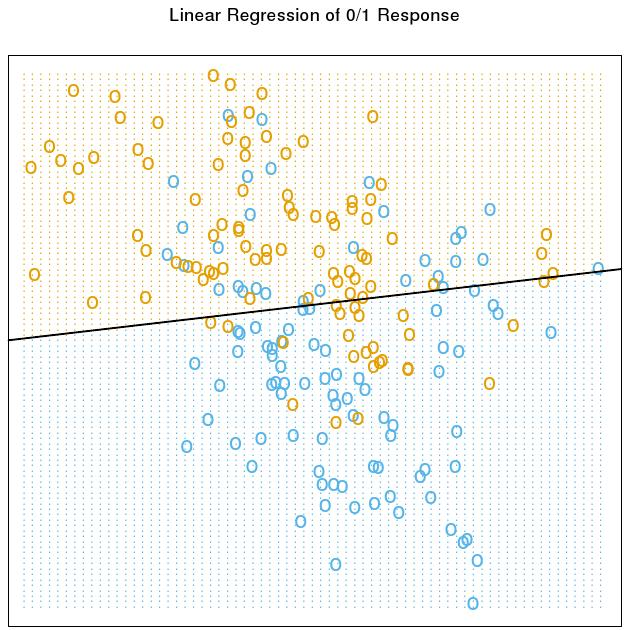
\includegraphics[width=.5\textwidth]{ex_mc.jpg}\\
    {\it \scriptsize
    Example of a binary classification problem in  $\mathbb{R}^2$. The 2 classes are coded as a binary 
    variable: \textcolor{orange}{ORANGE}=1, \textcolor{blue}{BLUE}=0. }
    \end{center}

\end{frame}


\subsection{Least Squares}

\begin{frame}
  \frametitle{Least Squares for classification}
  We seek a prediction model based on the linear regression of the outputs 
  $Y \in \{0,1\}$~:
  \begin{align*}
     Y & = X^T \boldsymbol{\beta} + \epsilon,
  \end{align*}

\begin{block}{Estimation of $\boldsymbol{\beta}$}
Minimize the training error rate (quadratic cost sense):
\begin{itemize}
%   \item $\hat{\boldsymbol{\beta}}=
%   \arg\min_{\boldsymbol{\beta}} RSS ( \boldsymbol{\beta} )$
 \item
 $
 RSS ( \boldsymbol{\beta} )
   = \sum_{i=1}^N (Y_i - X_i^T \boldsymbol{\beta} )^2 =
   (\boldsymbol{Y} - \boldsymbol{X} \boldsymbol{\beta})^T (\boldsymbol{Y} -
   \boldsymbol{X} \boldsymbol{\beta})$,\\
   where
   $\boldsymbol{Y}\in \mathbb{R}^N$ and $\boldsymbol{X}\in \mathbb{R}^{N\times 2}$
   are obtained by stacking the $Y_i$ and the $X_i^T$ respectively.
\end{itemize}

Using the orthogonality principle
\begin{align*}
   \hat{\boldsymbol{\beta}}&=
   (\boldsymbol{X}^T \boldsymbol{X} )^{-1} \boldsymbol{X}^T \boldsymbol{Y}  \quad \leftarrow
   \textrm{\it Least Squares Estimator}
\end{align*}
\end{block}

\begin{block}{Classification rule based on least squares regression}
\vspace{-2mm}
  \begin{align*}
     f(X) &= \begin{cases}
                0 \textrm{ if } \hat{Z}= X^T \hat{\boldsymbol{\beta}} \le 0.5,\\
                1 \textrm{ otherwise}
             \end{cases}
  \end{align*}

\end{block}


\end{frame}


\begin{frame}
  \frametitle{Least Squares for classification (Cont'd)}
  \begin{center}
    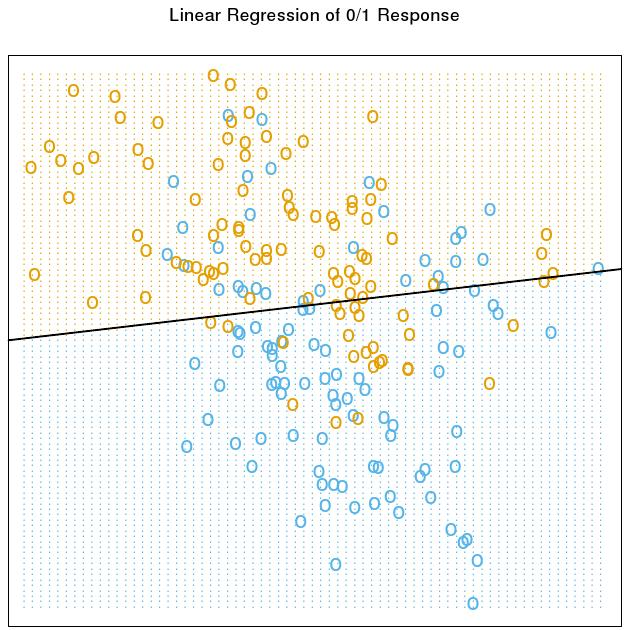
\includegraphics[width=.5\textwidth]{ex_mc.jpg}\\
    {\it \scriptsize
    Example of classification in $\mathbb{R}^2$. The 2 classes are coded as a binary variable: 
    \textcolor{orange}{ORANGE}=1, \textcolor{blue}{BLUE}=0. The line is the decision boundary 
    $x^T \widehat{\beta}= 0.5$: \textcolor{blue}{BLUE} decision region below, \textcolor{orange}{ORANGE} one above
    }
  \end{center}

\end{frame}

\subsection{k-NNB}

\begin{frame}
  \frametitle{'Black Box' method: $k$  Nearest-Neighbors ($k$-NN)}

  The prediction model is directly defined as:
  \begin{align*}
     \widehat{Y}(x) &= \frac{1}{k} \sum_{x_i \in N_k(x) } y_i,
  \end{align*}
  where $N_k(x) \equiv$ is the neighborhood of $x$ defined by the $k$ closest 
  inputs $X_i$ in the training sample.

  \begin{block}{Classification rule associated with $k$-NN}
  \vspace*{-5mm}
  \begin{align*}
     f(X) &= \begin{cases}
                1 \textrm{ if } \widehat{Y}(x) > \frac{1}{2},\\
                0 \textrm{ otherwise}
             \end{cases}
  \end{align*}
  $\Leftrightarrow$ majority vote among the $k$ closest neighbors
  of the testing point $x$
  \end{block}

  \begin{block}{Properties}
  %Intuitivement, on minimise le risque quadratique~:
  \vspace*{-5mm}
  \begin{align*}
     \hat{Y}(x) &= \textrm{ Average } \{ y_i | x_i \in  N_k(x) \} \approx E[Y | X=x ]
  \end{align*}
  But two approximations problematic in high dimension:
  \begin{itemize}
     \item Expectation $\leftarrow$ Average,
     \item Conditioning at a point  $\leftarrow$ conditioning on a neighborhood
  \end{itemize}

  \end{block}



\end{frame}


\begin{frame}
  \frametitle{K Nearest-Neighbors (Cont'd)}
  \begin{center}
    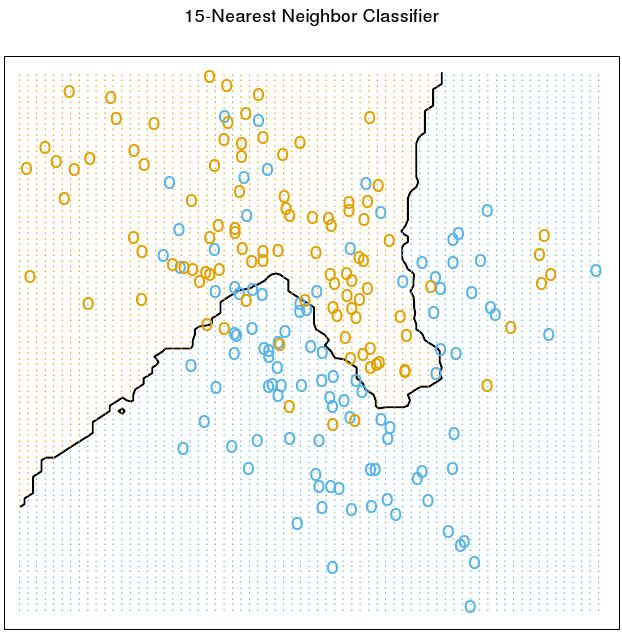
\includegraphics[width=.6\textwidth]{ex_kpp_15.jpg}
  \end{center}
\end{frame}

\subsection{Model Selection}

\begin{frame}
  \frametitle{Model complexity}
  Most of methods have a complexity related to their {\it effective} number of parameters

  \begin{block}{Linear regression: model order $p$}
  E.g. $d$th degree polynomial regression: $p=d+1$ parameters $a_k$ s.t.
    \begin{align*}
       Y &= \sum_{k=0}^d a_k x^{k} + \epsilon,\\
       &= \boldsymbol{X}_d \boldsymbol{a}_d + \epsilon,
    \end{align*}
    where
    \begin{align*}
       \boldsymbol{X}_d &= \left[x^0, x^1, \ldots, x^d\right], \\
       \boldsymbol{a}_d &= \left[a_0, a_1, \ldots, a_d\right]^T.
    \end{align*}

  \end{block}
\end{frame}

% \begin{frame}
%   \frametitle{Linear Regression}
%   \begin{block}{Polynomial order $p$ influence}
%   \end{block}
%   \begin{center}
%     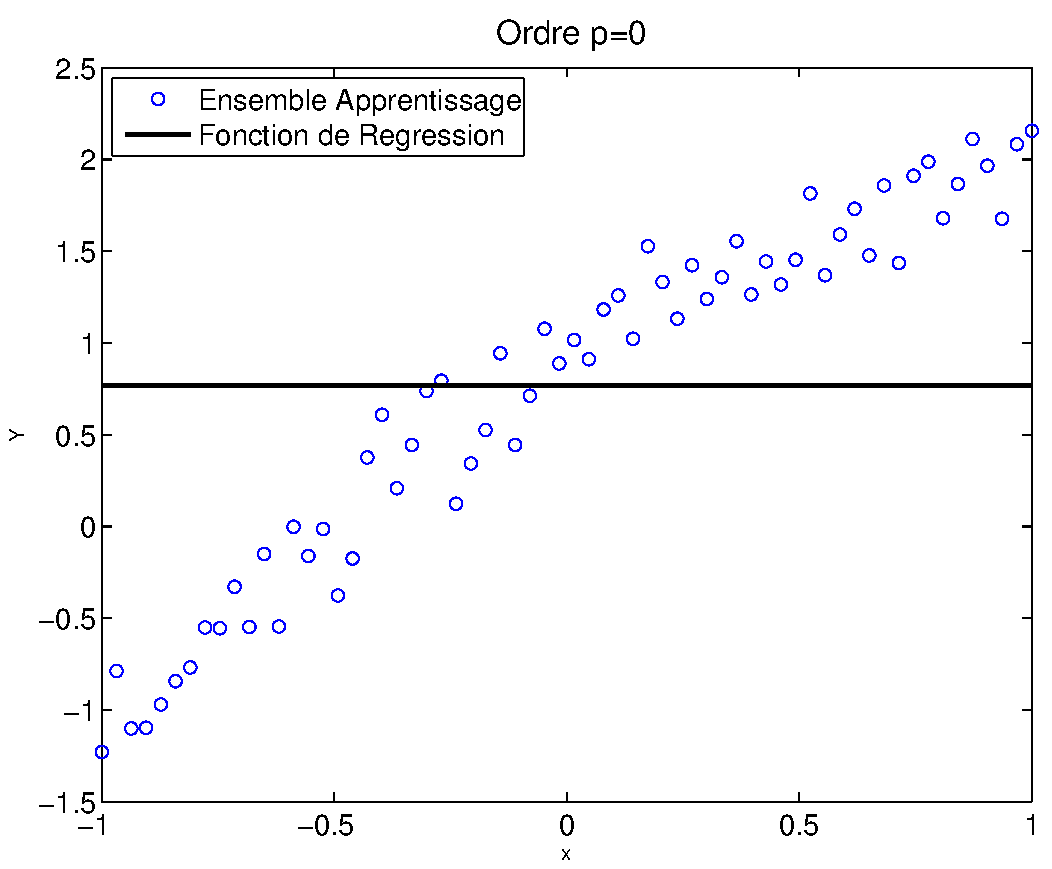
\includegraphics[width=.33\textwidth]{regression_order_00.pdf} \hfill
%     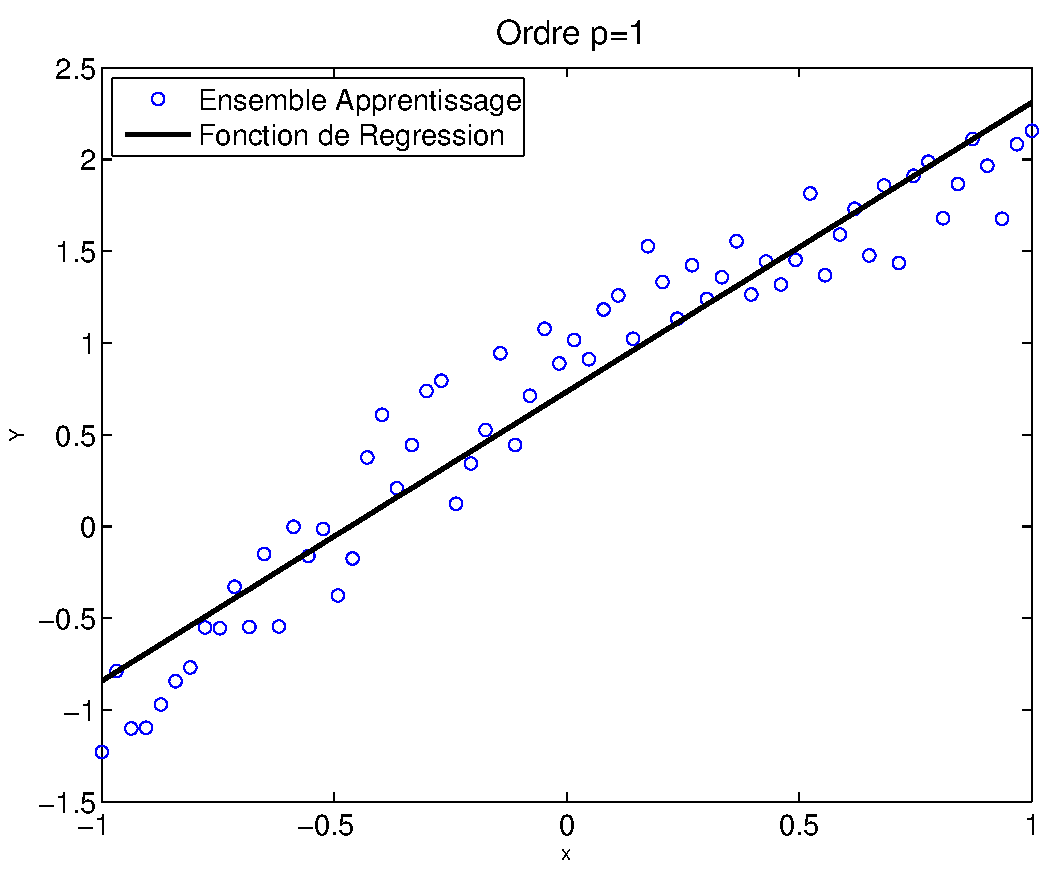
\includegraphics[width=.33\textwidth]{regression_order_01.pdf}\hfill
%     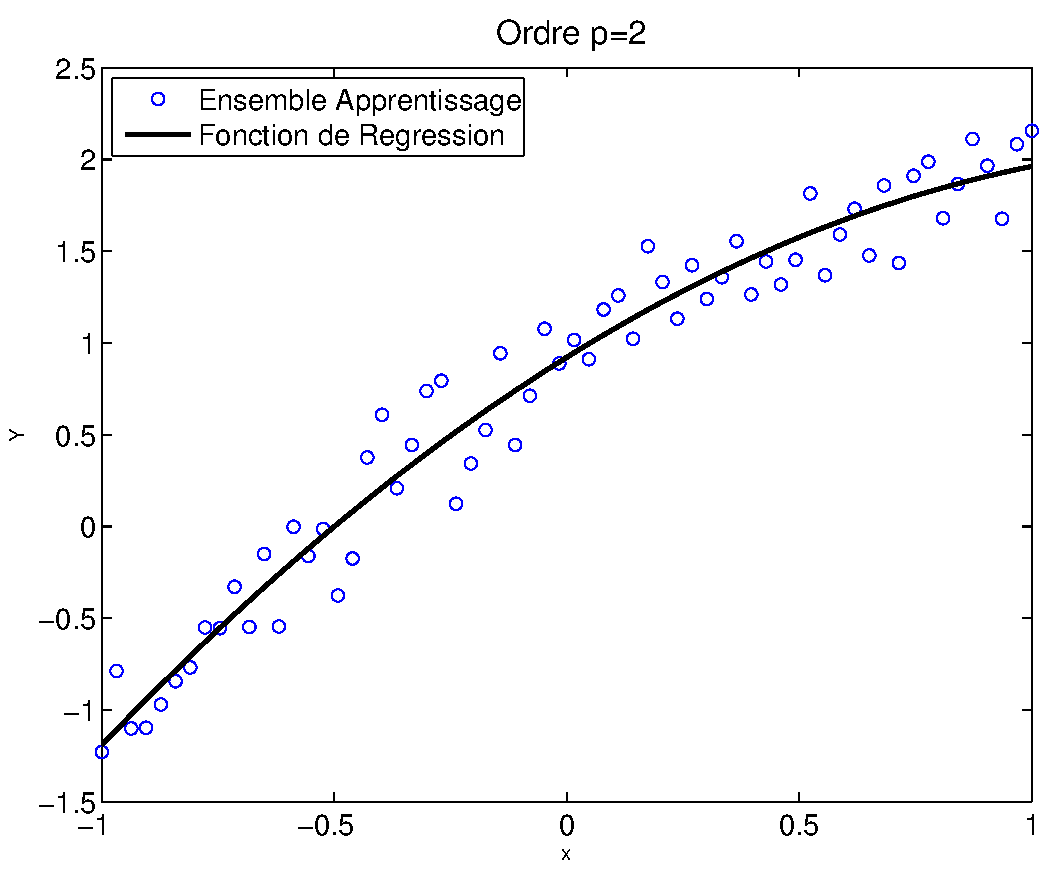
\includegraphics[width=.33\textwidth]{regression_order_02.pdf}\\
%     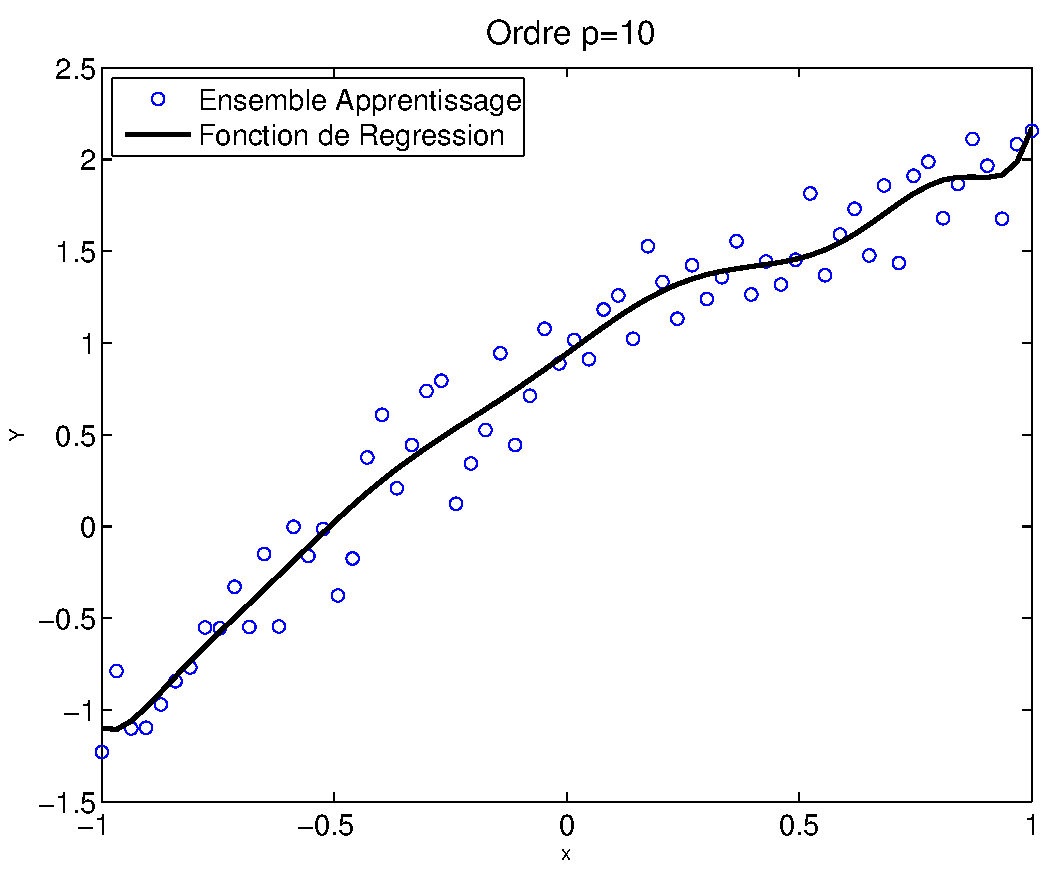
\includegraphics[width=.33\textwidth]{regression_order_10.pdf} \hfill
%     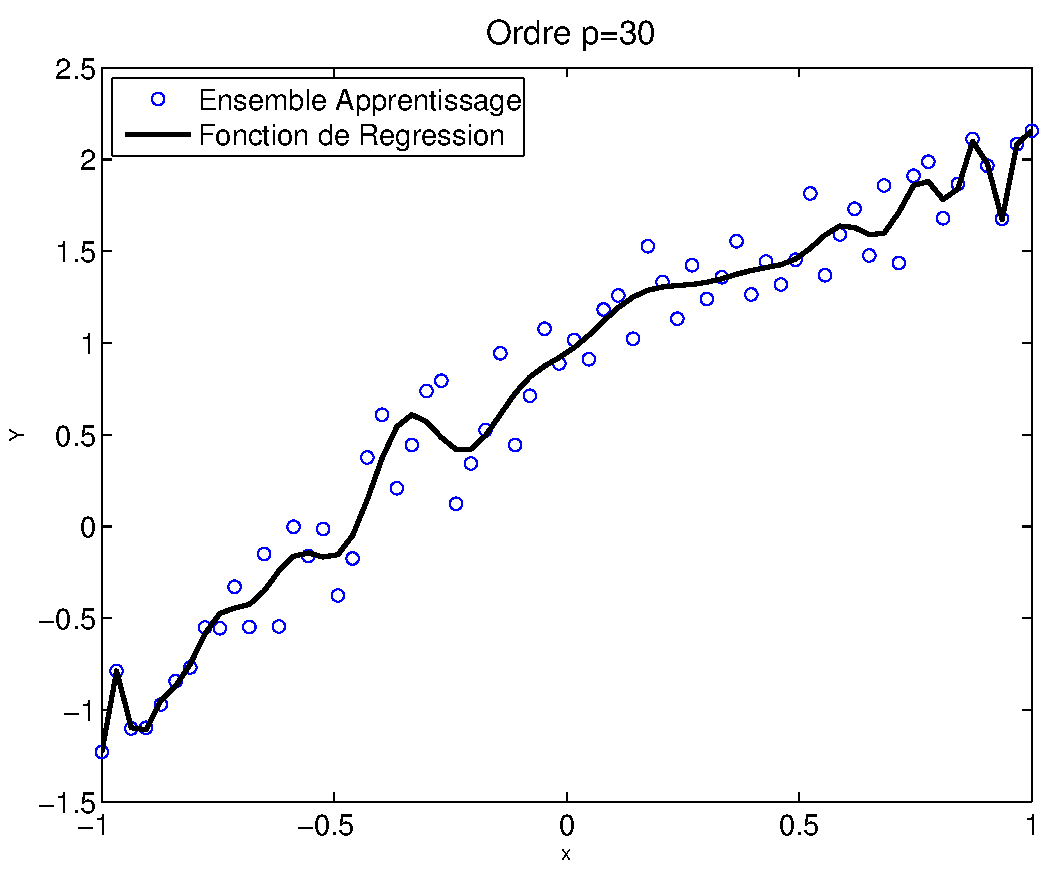
\includegraphics[width=.33\textwidth]{regression_order_30.pdf}\hfill
%     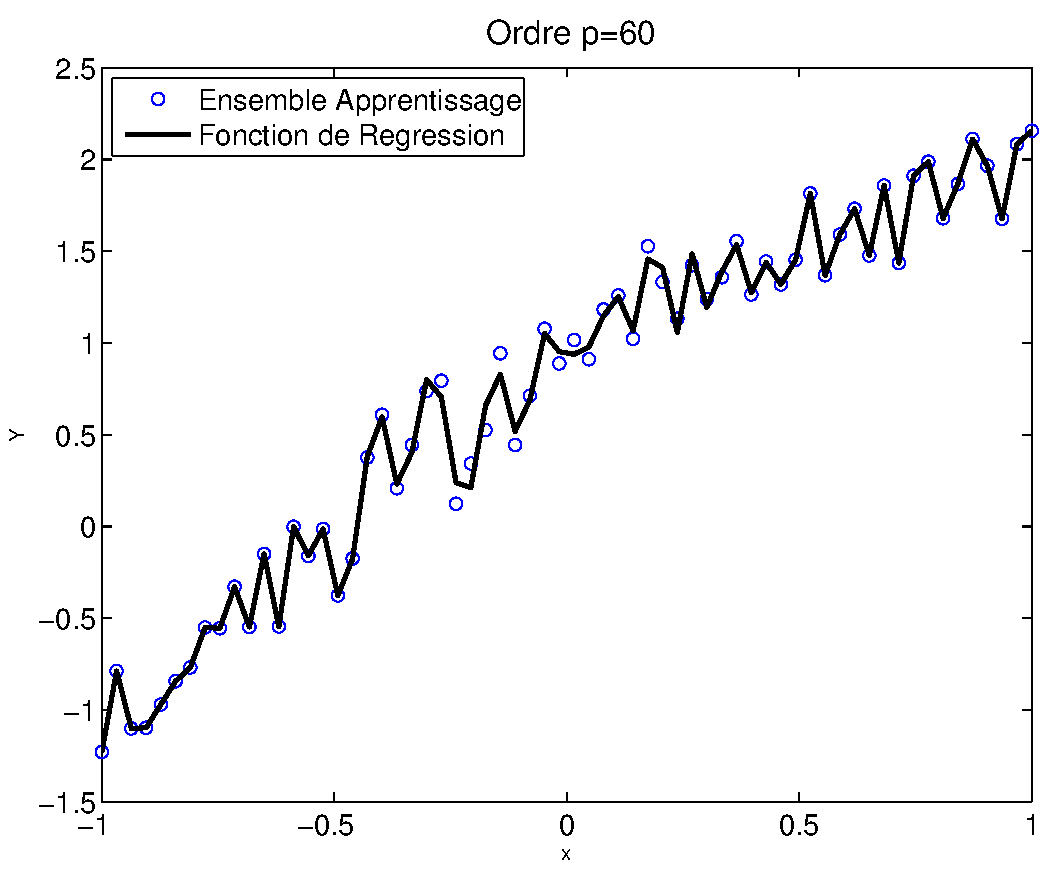
\includegraphics[width=.33\textwidth]{regression_order_60.pdf}
%   \end{center}
% \end{frame}

\begin{frame}
  \frametitle{Linear regression: complexity vs stability}
  \begin{block}{Polynomial degree $d$ influence  \alert{ $\leftarrow$ over-fitting issue} } %\visible<3>{ \alert{ $\leftarrow$ over-fitting} } }
  
  \end{block}
  
  \begin{center}
   %\begin{overprint}
    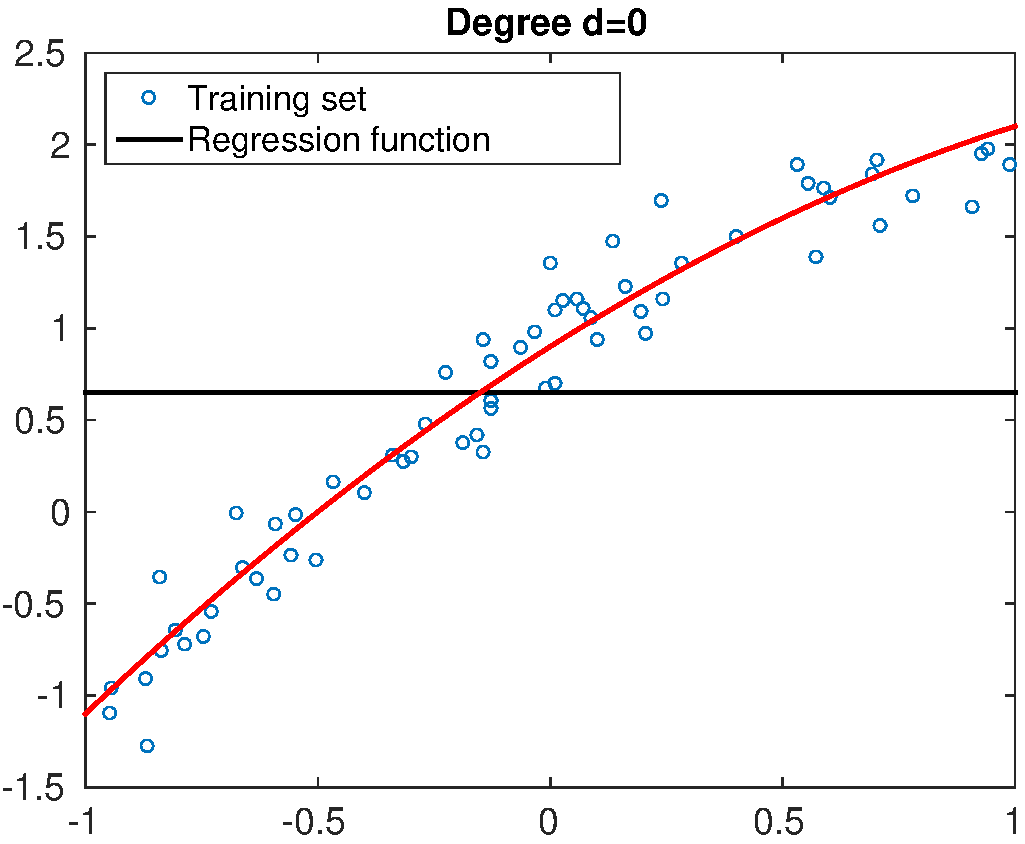
\includegraphics[width=.33\textwidth]{regression_order_regul_00_en.pdf} \hfill
    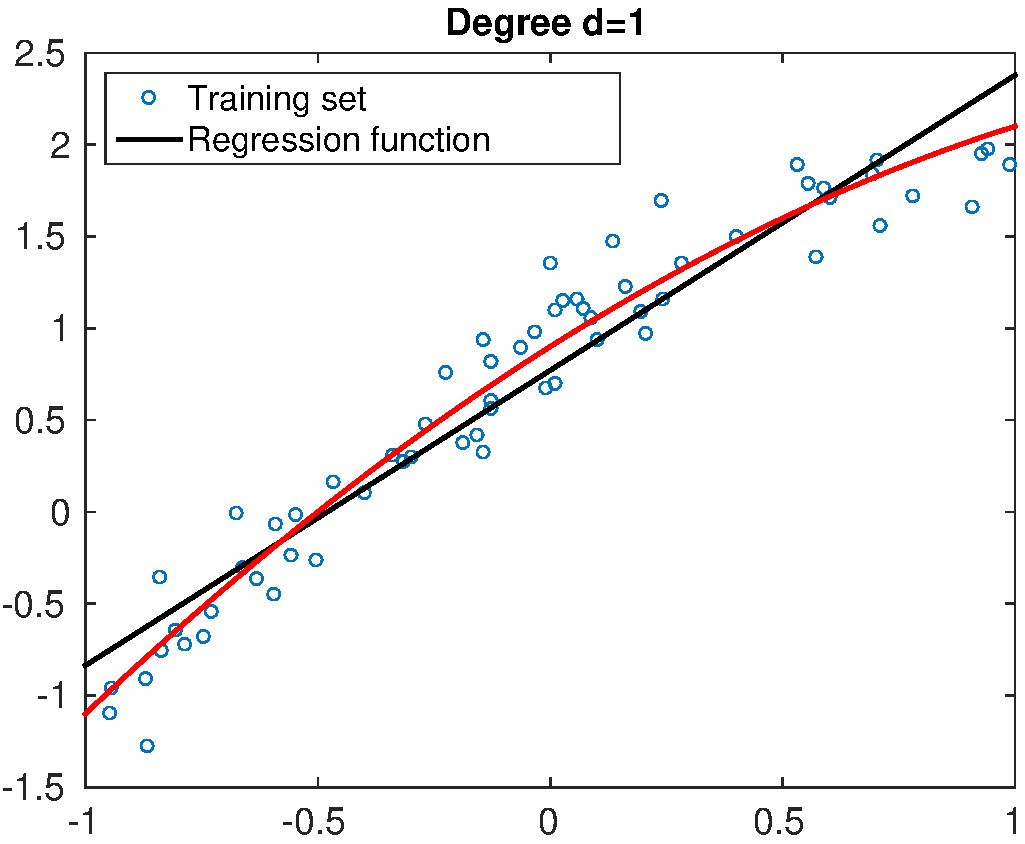
\includegraphics[width=.33\textwidth]{regression_order_regul_01_en.pdf}\hfill
    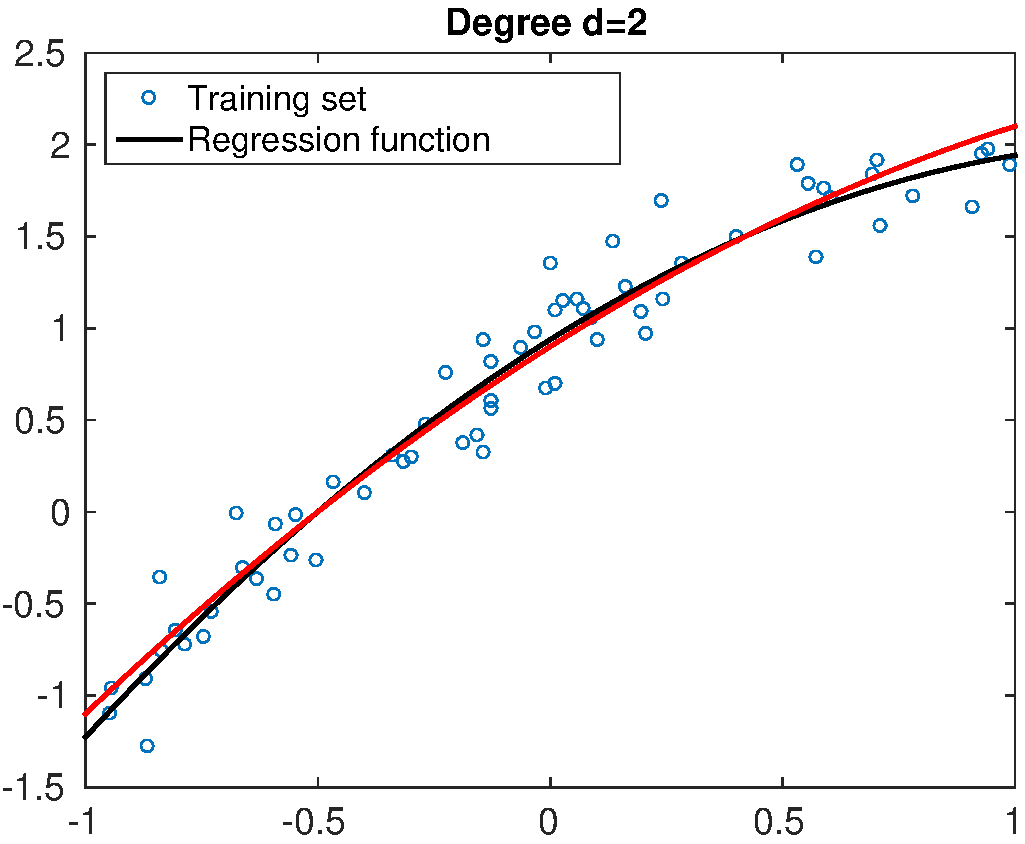
\includegraphics[width=.33\textwidth]{regression_order_regul_02_en.pdf}\\
    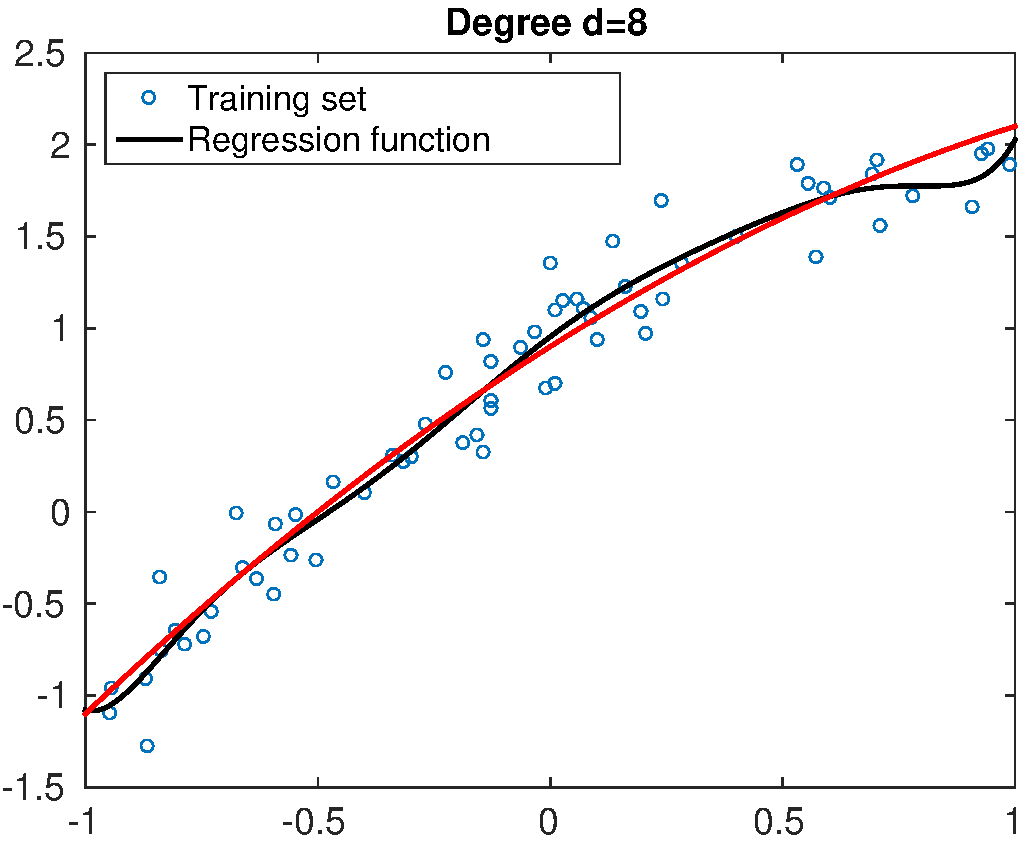
\includegraphics[width=.33\textwidth]{regression_order_regul_08_en.pdf} \hfill
    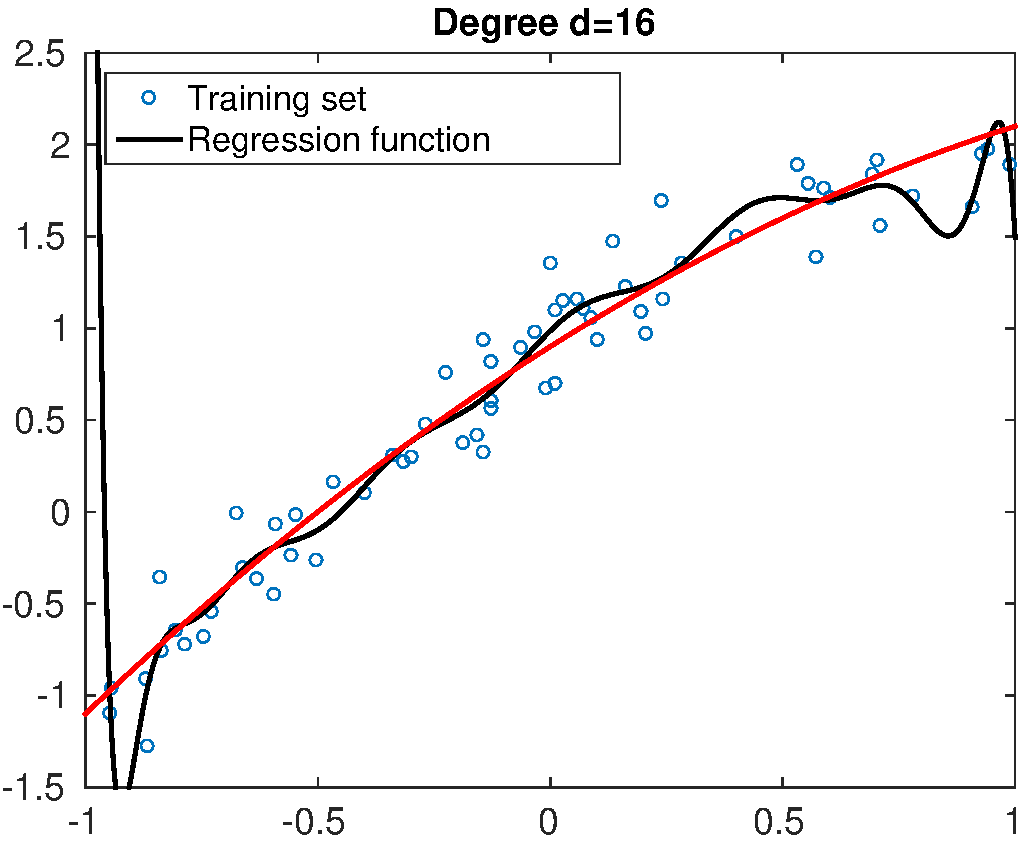
\includegraphics[width=.33\textwidth]{regression_order_regul_16_en.pdf}\hfill
    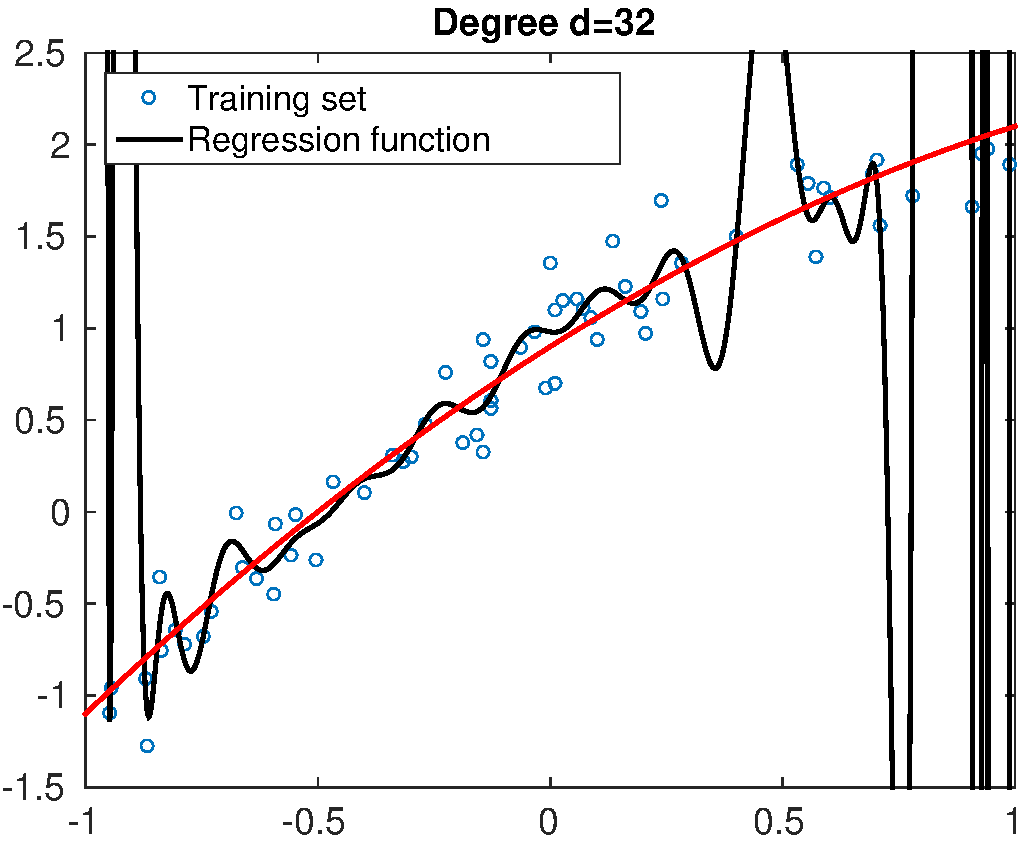
\includegraphics[width=.33\textwidth]{regression_order_regul_32_en.pdf}
    %\visible<2,3>{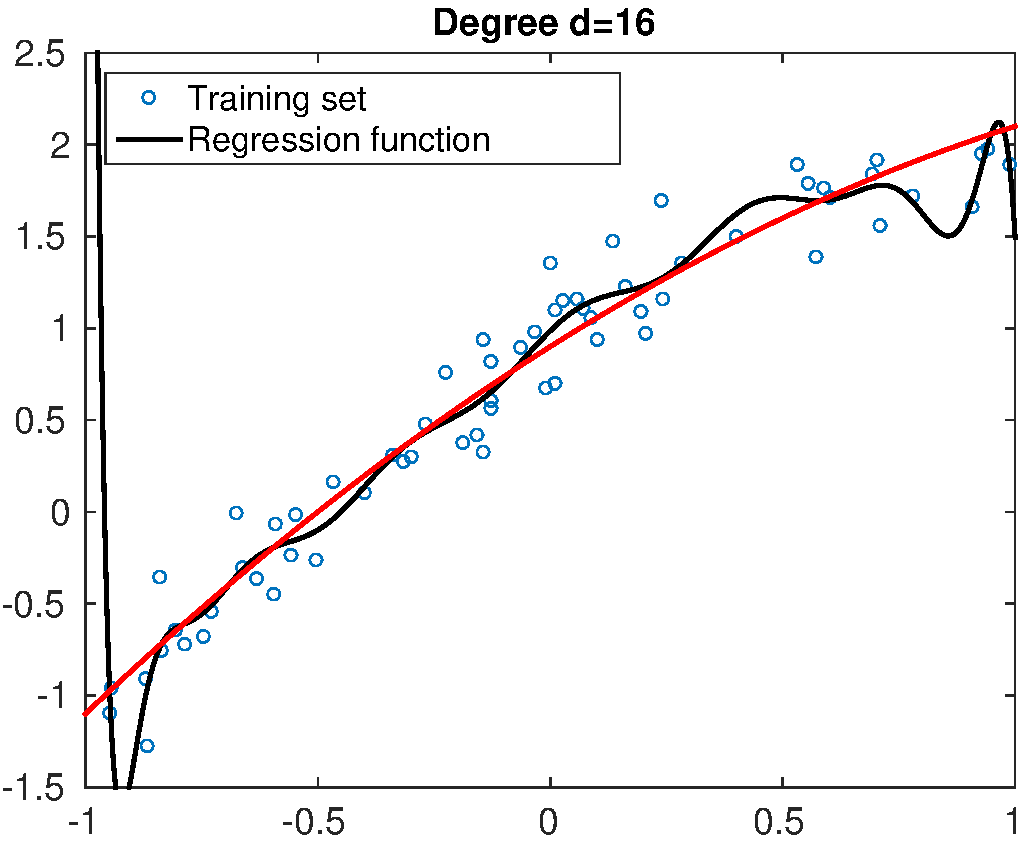
\includegraphics[width=.33\textwidth]{regression_order_regul_16_en.pdf}\hfill}
    %\visible<3>{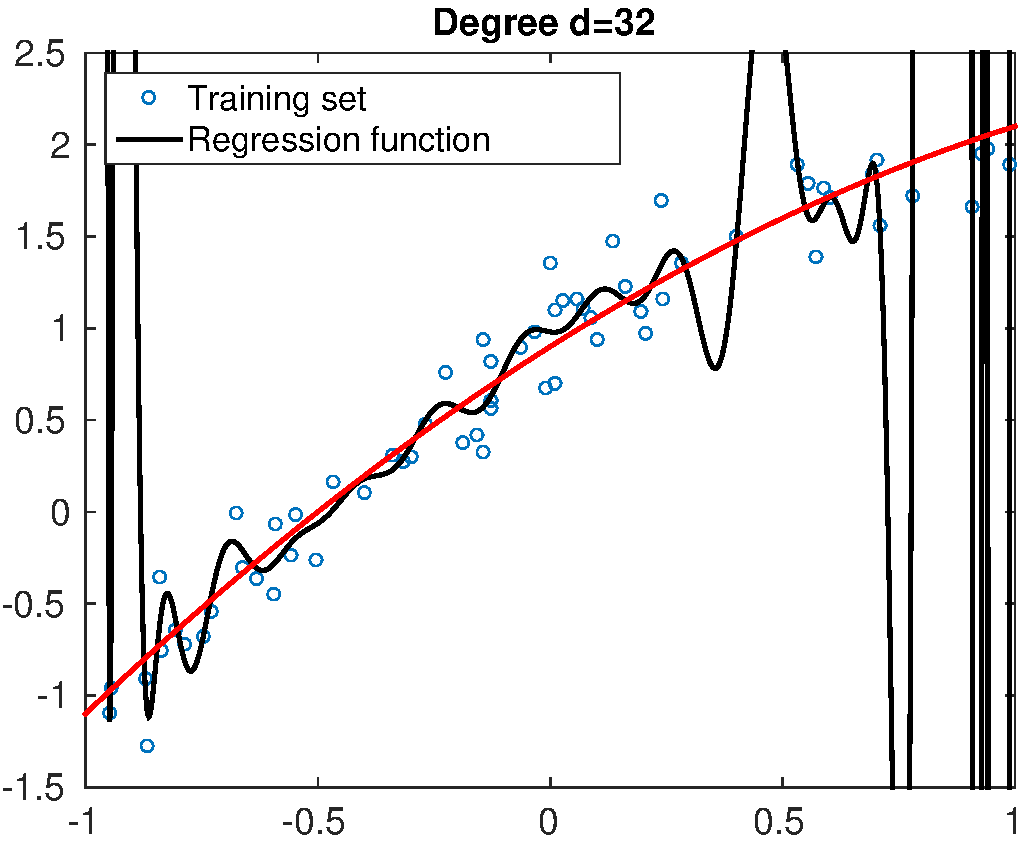
\includegraphics[width=.33\textwidth]{regression_order_regul_32_en.pdf}}
    %\end{overprint}
    \end{center}
\end{frame}

\begin{frame}
  \frametitle{Linear Regression (Cont'd)}
  \begin{block}{Error rate vs polynomial order $d$}
  \end{block}
  \begin{center}
    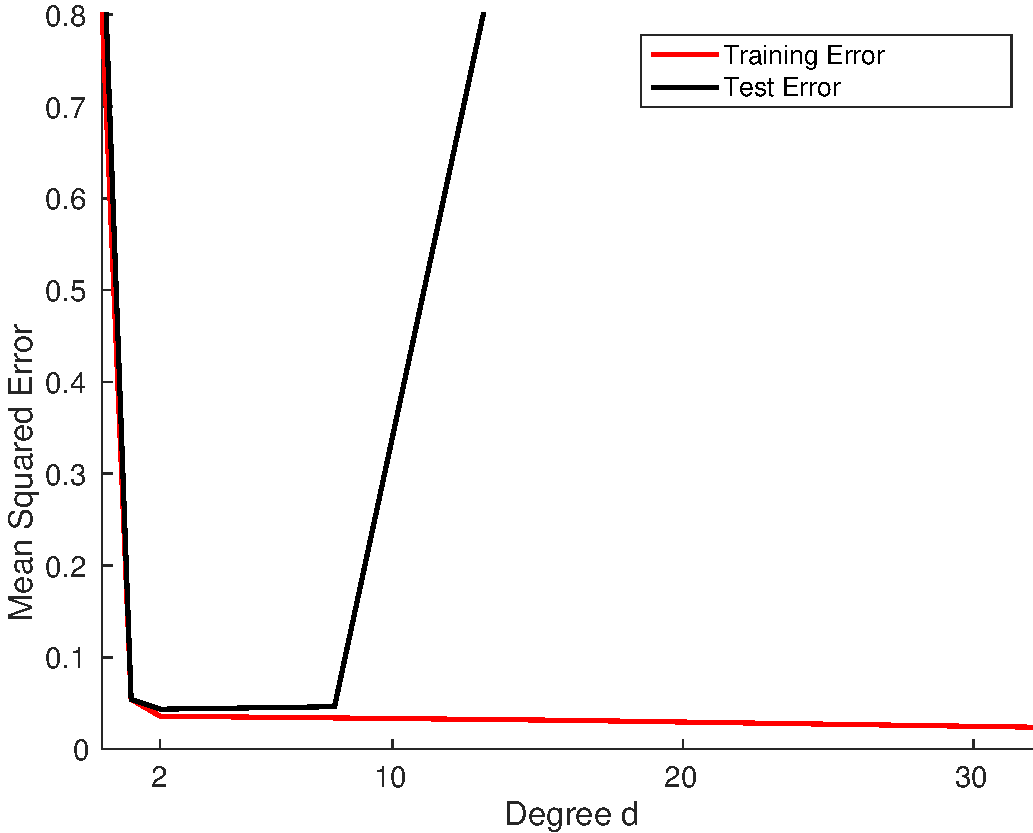
\includegraphics[width=.6\textwidth]{erreur_reg_vs_order_en.pdf}
  \end{center}
    \begin{itemize}
  \item True error rate minimized when $d=2$ ...
   \item ... true generative model: order $d=2$ polynomial (+ white noise)
  \end{itemize}
\end{frame}


\begin{frame}
  \frametitle{K Nearest-Neighbors}
%  \begin{block}{Nombre de Paramètres Effectifs $N_{\textrm{eff}} = \frac{N}{k}$ }
%  \end{block}
\begin{block}{$k$-NN: complexity parameter $k$}
      The effective number of parameters expresses as $N_{\textrm{eff}} = \frac{N}{k}$,
      where $N$ is the size of the training sample
  \end{block}

  \begin{center}
    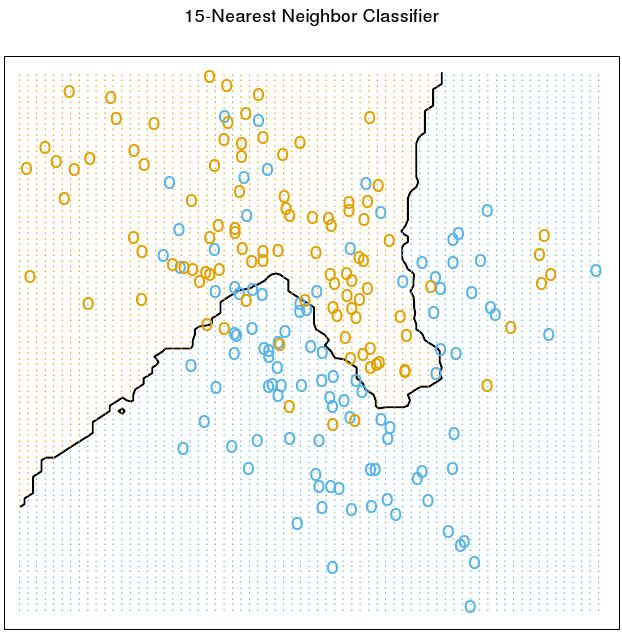
\includegraphics[width=.45\textwidth]{ex_kpp_15.jpg}
  \quad
    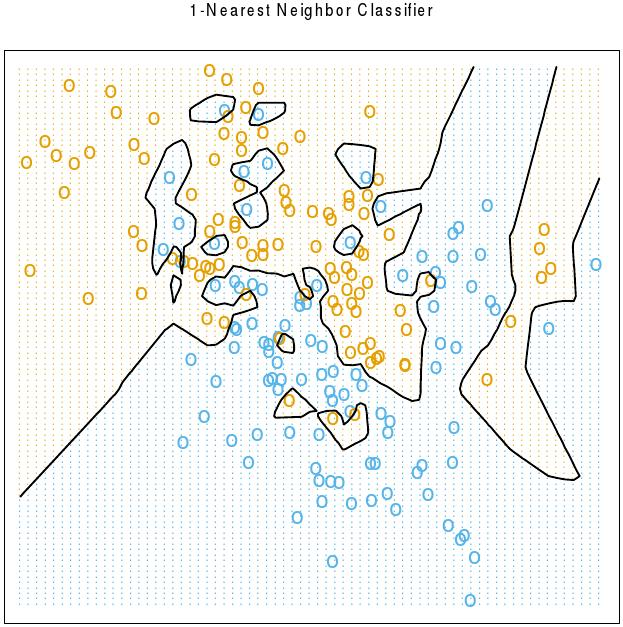
\includegraphics[width=.45\textwidth]{ex_kpp_1.jpg}\\
    $k=15$, $N_{\textrm{eff}} \approx 13$ \hspace{3cm} $k=1$, $N_{\textrm{eff}} \approx 200$
  \end{center}
  \begin{itemize}
     \item $k=1$ $\rightarrow$ training error is $0$ !
  \end{itemize}

\end{frame}


\begin{frame}
  \frametitle{Model Selection}
  \begin{center}
    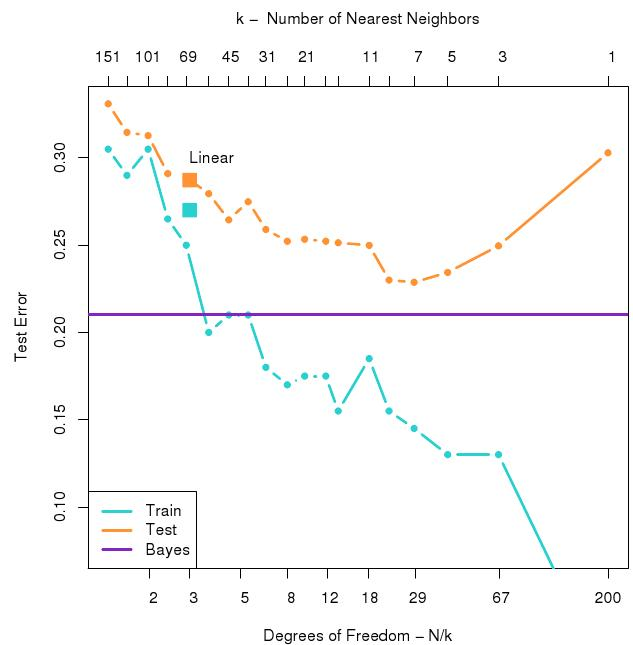
\includegraphics[width=.6\textwidth]{ex_selection_kpp_mc.jpg}
  \end{center}
\end{frame}


\begin{frame}
  \frametitle{Model Selection (Cont'd)}
  \begin{block}{Fundamental trade-off}
  \begin{itemize}
     \item too simple model (high bias) $\rightarrow$ \alert{under-fitting}
     \item too complex model (high variance) $\rightarrow$ \alert{over-fitting}
  \end{itemize}
  \end{block}
  \begin{center}
    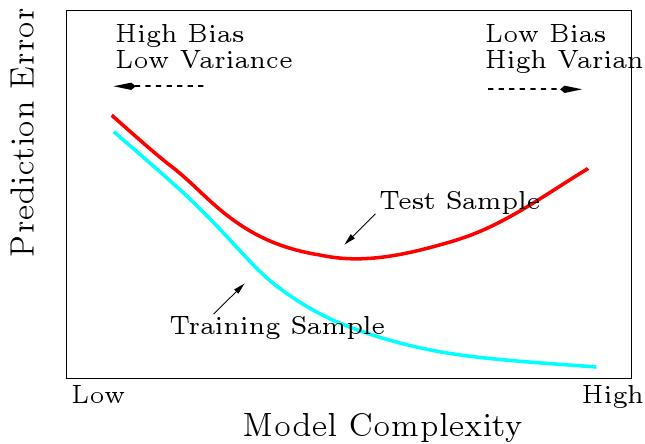
\includegraphics[width=.6\textwidth]{compromis.jpg}
  \end{center}
\end{frame}


\subsection{The truth on the example dataset}

\begin{frame}
  \frametitle{The (real) truth on the example dataset!}
  {\scriptsize
  \begin{block}{Generative model}
  \begin{itemize}
     \item For $k=1,\ldots,10$,  $\textcolor{orange}{m_k^1} \sim \mathcal{N}((0,1)^T,\boldsymbol{I} )$
     and $\textcolor{blue}{m_k^0} \sim \mathcal{N}((1,0)^T,\boldsymbol{I} ) $
      \item For $l=1,\dots,100$,  uniformly pick one $\textcolor{orange}{m_k^1}$, then draw $\textcolor{orange}{x_l^1} \sim \mathcal{N}(\textcolor{orange}{m_k^1},\boldsymbol{I}/5 )$
      %\quad \leftarrow$ \textcolor{orange}{ORANGE}
     \item Same for $\textcolor{blue}{x_l^0}$ with the  $\textcolor{blue}{m_k^0}$ \quad  ($N= 200$ for the training sample size)
     %\quad \leftarrow$ \textcolor{blue}{BLEU}
  \end{itemize}
  \end{block}
}
\vspace*{-4mm}
  \begin{center}
    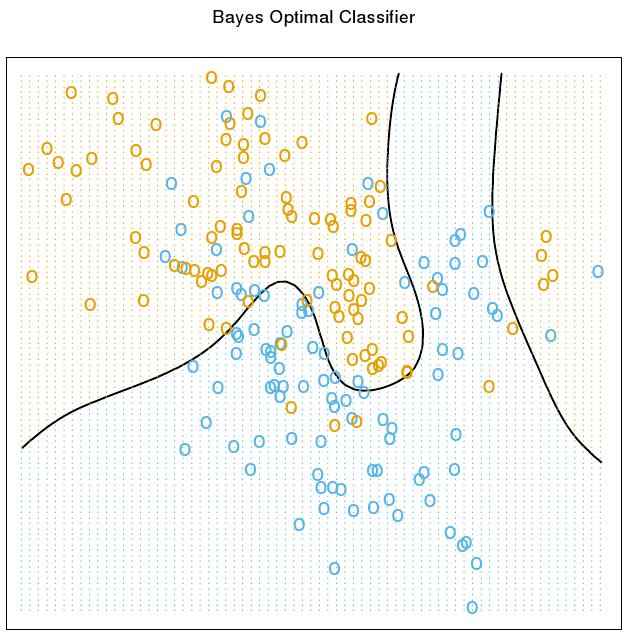
\includegraphics[width=.5\textwidth]{ex_bayes_class.jpg}
  \end{center}
\end{frame}








\end{document}
